\documentclass[conference]{IEEEtran}
\IEEEoverridecommandlockouts

\usepackage{cite}
\usepackage{amsmath,amssymb,amsfonts}
\usepackage{graphicx}
\usepackage{xcolor}
\usepackage{booktabs}
\usepackage{url}
\usepackage{hyperref}
\usepackage{tikz}
\usetikzlibrary{calc,positioning,arrows.meta,shapes.geometric}

\hypersetup{colorlinks=true,linkcolor=blue,citecolor=blue,urlcolor=blue}

\title{cursor-vibe-starter: An Auditable Workspace for\\AI-Directed Security Engineering}

\author{
\IEEEauthorblockN{Ali Murtaza Bhutto}
\IEEEauthorblockA{Independent Researcher\\
ORCID: 0009-0007-2787-943X\\
\href{https://github.com/thunderstornX/cursor-vibe-starter}{github.com/thunderstornX/cursor-vibe-starter}}
}

\begin{document}
\maketitle

\begin{abstract}
``Vibe coding'' --- the increasingly common practice of writing
software with an inline AI assistant in the loop --- has so far been
discussed primarily through productivity claims (``I shipped
\emph{N$\times$} faster''). This paper argues for a different framing:
the artefact left behind \emph{after} an AI-directed session ought to
include the rules the model was working under and the prompts the
human used, and the resulting codebase ought to be tagged at the
commit level so the share of AI-versus-human work can be derived
from the git log without resorting to style heuristics.
We present \texttt{cursor-vibe-starter}, an open-source reference
workspace built on this framing. The workspace ships a working
\texttt{.cursorrules} configuration, twelve five-part prompt
templates for security-engineering tasks, a complete worked example
(a FastAPI security microservice with a 20-test pytest suite), and a
single-file LOC analysis script that reports per-tag commit breakdowns
from the repository's own git log. We discuss why we deliberately
avoid productivity claims and describe the trade-offs of the
author-tagged measurement protocol.
\end{abstract}

\begin{IEEEkeywords}
AI-directed development, prompt engineering, Cursor IDE, software
methodology, security engineering, FastAPI
\end{IEEEkeywords}

% ----------------------------------------------------------------------
\section{Introduction}
\label{sec:intro}

A pattern has emerged in 2025--2026 software engineering: a developer
sits in front of a code editor with an inline LLM assistant, gives it
short natural-language instructions, reviews the resulting patches,
and ships the diff. Adoption is uneven; published methodology is more
uneven still. The literature on this practice is dominated by
productivity claims (``$N\times$ faster'', ``$M\%$ of my code is now
AI-written'') that are typically self-reported, rarely controlled,
and almost never reproducible.

This paper takes a smaller bite. We do not measure speedup. We
propose --- and ship working artefacts for --- a discipline under
which a codebase produced this way is itself a record of how it was
produced:

\begin{itemize}
\item The IDE-level rules the model was working under are committed
to the repository (\texttt{.cursorrules}).
\item The prompt library the human used is committed to the
repository, with each prompt's pitfalls section drawn from real
``the model produced this and I had to fix it'' experience.
\item Every commit in the repository is tagged at message level
(\texttt{[ai]}, \texttt{[manual]}, \texttt{[mixed]}, \texttt{[tooling]},
\texttt{[merge]}); a single-file script aggregates these into a
public LOC table.
\end{itemize}

\noindent\textbf{Contributions.} (i) An opinionated, open-source
\texttt{.cursorrules} for security-engineering work; (ii) a library
of twelve prompt templates with a strict five-part structure;
(iii) a complete worked-example FastAPI microservice exercising
JWT auth, Redis-backed rate limiting, and structured logging, with
a 20-test pytest suite that all pass; (iv) a measurement protocol
based on author-tagged commits, with the rationale for why we
avoid style-based AI-detection heuristics.

\begin{figure}[t]
\centering
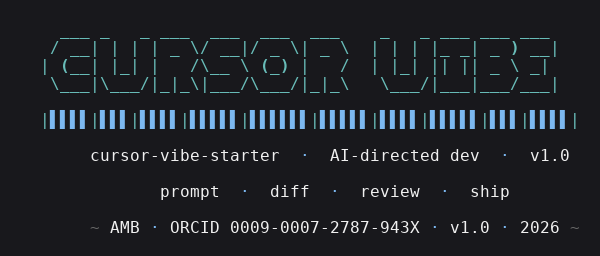
\includegraphics[width=0.95\columnwidth]{figures/banner.png}
\caption{The repository banner. ``Vibe coding'' is the input; the
audit-friendly artefact-with-protocol is the output.}
\label{fig:banner}
\end{figure}

% ----------------------------------------------------------------------
\section{Workspace Architecture}
\label{sec:arch}

The repository has three top-level deliverables:

\subsection{The \texttt{.cursorrules} file}

A single Markdown file in the repo root that the Cursor IDE feeds to
the model on every session. It encodes the project's stance on:
\textbf{style} (Python 3.10+, type hints everywhere, comments
explain ``why'' not ``what'');
\textbf{security} (no hardcoded secrets, parameterised SQL, JWT
\texttt{algorithms=[ALG]} as a list to defeat alg-confusion, never
log a request body);
\textbf{testing} (every public function gets a pytest test, mock the
wire not the function under test);
\textbf{frameworks} (FastAPI, pydantic v2, httpx, pytest); and
\textbf{response format} (lead with the change, flag security-relevant
decisions, no marketing language).

\subsection{The prompt library}

Twelve numbered Markdown files, each a copy-pasteable template
covering a discrete security-engineering task: API design, security
review, test generation, container packaging, schema design, JWT
auth, error handling, structured logging, CI pipeline,
maintainability refactor, documentation, and incident-response
tooling.

Every template enforces the same five-part structure:

\begin{enumerate}
\item \textbf{Context} --- when this prompt is the right one to reach
for.
\item \textbf{Template} --- the actual prompt with
\texttt{\{placeholders\}} for project-specific details.
\item \textbf{Example} --- a filled-in example showing real usage.
\item \textbf{Expected Output} --- what good output looks like.
\item \textbf{Common Pitfalls} --- failure modes drawn from real
production experience with the prompt.
\end{enumerate}

Crucially, the \emph{Common Pitfalls} section is what differentiates
this library from a generic prompt collection. Each entry there is
a documented model failure. For example,
\texttt{prompts/06\_auth\_flow.md}'s pitfalls section explicitly
warns about \texttt{algorithms=ALGORITHM} (a string) versus
\texttt{algorithms=[ALGORITHM]} (a list) --- because PyJWT silently
accepts \emph{any} algorithm if the parameter is a string, which is
the canonical JWT alg-confusion exploit.

\subsection{The worked example}

\texttt{example/security-microservice/} is a complete FastAPI
service whose architecture is summarised in
Fig.~\ref{fig:service-arch}. Twenty pytest cases cover the auth
path, scan endpoints, rate limiter, log redaction, and health
probe. The full suite runs in $\sim$3 seconds.

\begin{figure}[t]
\centering
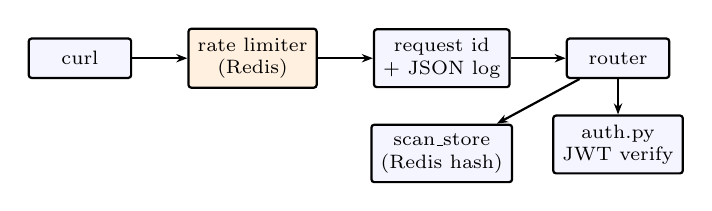
\begin{tikzpicture}[
    node distance=0.45cm and 0.7cm,
    every node/.style={font=\scriptsize},
    nd/.style={rectangle, rounded corners=1pt, draw=black, thick,
               minimum width=1.3cm, minimum height=0.50cm,
               align=center, fill=blue!4},
    side/.style={rectangle, rounded corners=1pt, draw=black, thick,
                 minimum width=1.3cm, minimum height=0.50cm,
                 align=center, fill=orange!12},
    arr/.style={-{Stealth[length=4pt]}, thick}
]
\node[nd]                          (cli)   {curl};
\node[side, right=of cli]          (rl)    {rate limiter\\(Redis)};
\node[nd, right=of rl]             (rid)   {request id\\+ JSON log};
\node[nd, right=of rid]            (rt)    {router};
\node[nd, below=of rt]             (auth)  {auth.py\\JWT verify};
\node[nd, below=of rid]            (svc)   {scan\_store\\(Redis hash)};
\draw[arr] (cli)  -- (rl);
\draw[arr] (rl)   -- (rid);
\draw[arr] (rid)  -- (rt);
\draw[arr] (rt)   -- (auth);
\draw[arr] (rt)   -- (svc);
\end{tikzpicture}
\caption{Request lifecycle through the worked-example service.
Outer-most middleware is rate limiting; auth is a route-level
dependency so unauth'd \texttt{/health} stays cheap.}
\label{fig:service-arch}
\end{figure}

\begin{table}[t]
\centering
\caption{Worked-example endpoints and their stable error codes.}
\label{tab:endpoints}
\renewcommand{\arraystretch}{1.18}
\begin{tabular}{llll}
\toprule
\textbf{Method} & \textbf{Path}             & \textbf{Auth}   & \textbf{Error codes} \\
\midrule
GET             & /health                   & none            & ---                  \\
POST            & /v1/auth/login            & none            & auth.bad\_credentials \\
POST            & /v1/scans                 & Bearer          & request.invalid, rate.limited \\
GET             & /v1/scans/\{id\}          & Bearer          & scan.not\_found      \\
GET             & /v1/scans                 & Bearer          & ---                  \\
\bottomrule
\end{tabular}
\end{table}

% ----------------------------------------------------------------------
\section{Measurement Protocol}
\label{sec:method}

We claim no productivity multiplier. We do propose a transparent,
gameable, but \emph{honest} record of which lines in a release came
through which workflow.

Each commit's first line begins with one of five tags:
\texttt{[ai]} (AI-directed: prompt $\rightarrow$ patch $\rightarrow$
review),
\texttt{[manual]} (human-typed),
\texttt{[mixed]} (collaboration where neither dominates),
\texttt{[tooling]} (generated configs, lockfiles, CI yaml; bucketed
separately because LOC ratios from generated text say nothing about
effort), or
\texttt{[merge]} (merge commit with no original content; excluded
from totals). Untagged commits land in an \texttt{[untagged]} bucket
that exists to make discipline drift visible rather than silently
inflating one of the other buckets.

\texttt{metrics/loc\_analysis.py} parses the repository's
\texttt{git log}, computes per-commit \texttt{insertions $-$ deletions}
over tracked source files (excluding vendored, generated, and binary
paths), and aggregates by tag. Output formats: text table,
GitHub-flavoured markdown, JSON.

\subsection{Why no AI-style heuristics?}

It is tempting to write a clever script that infers ``AI lines'' from
docstring length, type-hint density, or naming patterns. We
considered and rejected this approach for three reasons:

\begin{enumerate}
\item \textbf{Circularity.} The most reliable AI-style fingerprints
are those of the \emph{current} model generation; they break the
moment a different model with a different style is used.
\item \textbf{Gaming.} A heuristic that flags ``AI'' on long
docstrings rewards rewriting docstrings, which is busywork that
doesn't change the underlying question.
\item \textbf{Hidden tail.} Real AI-pair-coded codebases contain a
lot of short functions and one-line wires --- exactly the cases
heuristics miscount. The honest answer is ``the author tells you''.
\end{enumerate}

The author-tagged protocol is the same trade-off used in academic
authorship lists: contributors say what they contributed, and the
report aggregates. If the author tags wrong, the report is wrong;
that is a feature, because it forces honesty rather than rewarding
clever metric-gaming.

% ----------------------------------------------------------------------
\section{Limitations}
\label{sec:limits}

\textbf{No effort tracking.} A 50-line \texttt{[ai]} patch that took
two hours of human review counts identically to one the human waved
through. The metric measures \emph{output}, not \emph{effort}.

\textbf{Autocomplete blur.} Modern editors complete tokens and short
lines automatically. The threshold for \texttt{[ai]} in this protocol
is ``the patch was written by the model, not the cursor''. That is
judgment, not measurement.

\textbf{Refactor invisibility.} A \texttt{[manual]} refactor that
nets to zero LOC reports zero. Refactors should be inspected
separately if effort is the question.

\textbf{Single-author bias.} The protocol works as written for a
single-author repo or a small team with shared discipline. A larger
team would need a code-review-time tag-enforcement step or the
discipline drifts.

% ----------------------------------------------------------------------
\section{Reproducibility}
\label{sec:repro}

The repository is released under the MIT licence. The
\texttt{.cursorrules} file, the twelve prompts, and the worked-example
service are deposited at every release tag; a fresh clone will
reproduce all 20 pytest cases in $\sim$3 seconds and all four
DevSecOps gates (Bandit medium-or-higher, pip-audit, Semgrep
\texttt{p/python} + \texttt{p/security-audit}, plus
no-AI-attribution-trace audit) clean. This release is archived at
\texttt{10.5281/zenodo.20480451}.

% ----------------------------------------------------------------------
\section*{Acknowledgement}

This work cites and complements the OSINT-legal framework
in~\cite{bhutto2025osintlegal}, applied here to the question of
recording and disclosing AI involvement in shipped software.

\begin{thebibliography}{1}
\bibitem{cursor2024}
Cursor, ``Cursor IDE Documentation,''
\url{https://cursor.sh/docs}, 2024 (accessed 2026).

\bibitem{bhutto2025osintlegal}
A.~M.~Bhutto, ``Operationalising the OSINT Lifecycle: A Framework
for Privacy-Aware and Compliant OSINT Operations,'' Zenodo, 2025.
\href{https://doi.org/10.5281/zenodo.16924934}{doi:10.5281/zenodo.16924934}

\bibitem{owasp-llm-2025}
OWASP, ``Top 10 for Large Language Model Applications,'' 2025
revision, \url{https://owasp.org/www-project-top-10-for-large-language-model-applications/}.

\bibitem{pyjwt}
J.~Padilla et al., ``PyJWT,''
\url{https://pyjwt.readthedocs.io}, 2024 (accessed 2026).
\end{thebibliography}

% Cursor-shaped colophon.
\vspace{0.4em}
\begin{center}
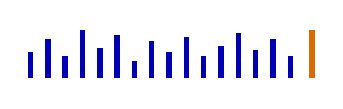
\begin{tikzpicture}[scale=0.55]
% audio-waveform bar
\foreach \x/\h in {0/0.6, 0.4/0.9, 0.8/0.5, 1.2/1.1, 1.6/0.7, 2.0/1.0,
                    2.4/0.4, 2.8/0.85, 3.2/0.6, 3.6/0.95, 4.0/0.5,
                    4.4/0.75, 4.8/1.05, 5.2/0.65, 5.6/0.9, 6.0/0.5}{
  \draw[line width=2.0pt, blue!70!black] (\x, 0) -- (\x, \h);
}
% blinking caret to the right of the bar
\draw[line width=2.0pt, orange!85!black] (6.5, 0) -- (6.5, 1.1);
\end{tikzpicture}\\[0.2em]
{\footnotesize\itshape ~AMB \(\cdot\) ORCID 0009-0007-2787-943X
\(\cdot\) v1.0 \(\cdot\) 2026~}
\end{center}

\end{document}
